\section{Ergonomische Verbesserungen}

Dieser Teil wird sich auf die Implementierung einiger Lösungen für das im Abschnitt \ref{sec:analyse-ergo} erwähnte Problem konzentrieren.
Diese Lösungen basieren hauptsächlich auf den Eigenschaften der Angular-Frameworks, die im Abschnitt \ref{sec:angular} beschrieben wurden.

\subsection{animierte Illustrationen}

Eine interessante Herausforderung war die Erstellung von animierten Illustrationen, die eine sympathischere Schnittstellenbildung ermöglichten.
Dazu wurden Angular-Komponenten entwickelt, die aus \ac{SVG}-Vorlagen mit \ac{CSS}-Stilen und -Animationen bestehen, um bestimmte Bereiche des \ac{SVG} zu animieren.
Die SVGs wurden mit der Figma-Software so erstellt, dass einige Teile der endgültigen SVGs eine eindeutige \ac{HTML}-ID mithilfe der Syntax \lstinline{id="identifer"} haben.

\begin{lstlisting}[
  language=html,
  caption={Vereinfachtes SVG der Illustration der Seite 404 (siehe Abbildung \ref{fig:app_404_new})},
  captionpos=b,
  label={lst:wifi_illustration_svg}
]
<svg xmlns="http://www.w3.org/2000/svg" width="906" height="1006" viewBox="0 0 906 1006" fill="none">
  <g id="404">
    <g id="wifi">
      <path id="wave-3" d="M651.095 135.65C578.316 109.161 ..."/>
      <path id="wave-2" d="M613.188 239.798C579.397 227.499 ..."/>
      <path id="wave-1" d="M576.311 341.191C596.659 348.597 ..."/>
    </g>
    ...
\end{lstlisting}

\begin{lstlisting}[
  language=css,
  caption={Vereinfachter \ac{SASS}-Code, um das WIFI-Logo wie eine Welle zu animieren, die in der \ac{SVG} \ref{lst:wifi_illustration_svg} enthalten ist},
  captionpos=b
]
#wifi {
  [id^=wave] {
    animation: signal-wave 2s infinite;
  }

  #wave {
    &-2 { animation-delay: .2s; }
    &-3 { animation-delay: .4s; }
  }
}

@keyframes signal-wave {
  0% { opacity: 0; }
  60% { opacity: 1; }
  100% { opacity: 0; }
}
\end{lstlisting}

Insgesamt wurden 4 animierte Illustrationen erstellt, die über einen externen Link zum Service JSFiddle zugänglich sind.

\begin{table}[H]
  \begin{tabular}{p{0.5\linewidth} | p{0.5\linewidth}}
    Name der Komponente                                 & Link zur Vorschau                                                                               \\ \hline\hline

    \textbf{app-animated-illustration-peacefull-forest} & \href{https://jsfiddle.net/johannchopin/Lwu0nvm3/}{https://jsfiddle.net/johannchopin/Lwu0nvm3/} \\\hline
    \textbf{app-animated-illustration-404}              & \href{https://jsfiddle.net/johannchopin/puj3es5q/}{https://jsfiddle.net/johannchopin/puj3es5q/} \\\hline
    \textbf{app-animated-illustration-access-denied}    & \href{https://jsfiddle.net/johannchopin/pgkh0rfL/}{https://jsfiddle.net/johannchopin/pgkh0rfL/} \\\hline
    \textbf{app-animated-illustration-site-not-found}   & \href{https://jsfiddle.net/johannchopin/30js2zpr/}{https://jsfiddle.net/johannchopin/30js2zpr/}
  \end{tabular}
  \caption{Aktionen, die der Nutzer im Rahmen von Usability-Tests durchführen muss}
\end{table}

Diese Illustrationen können dann leicht in andere Seiten-Templates integriert werden:

\begin{lstlisting}[
  language=html,
  caption={Integration einer animierten Illustration bei einer falschen Eingabe der \textit{Site}-ID durch den Benutzer},
  captionpos=b
]
<div *ngIf="invalidSiteId">
  <app-animated-illustration-site-not-found></app-animated-illustration-site-not-found>
  <h2 class="bold">Site Not Found</h2>
  <p class="text-center">
    The site you're looking for might be removed or might never exist on earth.
  </p>
  ...
</div>
\end{lstlisting}


\subsection{Service für blinkende Favicons}

Die Animation des Favicons der Anwendung wird mithilfe eines Angular Service verwaltet, damit es von allen Komponenten der Anwendung konsumiert werden kann.
Dazu werden die beiden Favicons \textit{default.icon} und \textit{danger.ico} im Ordner \textit{src/assets/favicons} gespeichert.
Der \textit{assets}-Ordner in einem Angular-Projekt wird von der Rückgabe so bedient, dass Sie einfach auf die Favicons in der Anwendung zugreifen können, indem Sie den URI \textit{/favicons/default.ico} verwenden.
Der benutzerdefinierte Dienst \lstinline{FaviconService} wird den Dienst \lstinline{NgxFaviconService} verwenden, um einfach den Favicon-Link der Anwendung mithilfe seiner \lstinline{setCustomFavicon}-Methode zu bearbeiten.

Dieser verfügt über eine \lstinline{blink}-Methode, mit der zwei Favicons, die als Parameter übergeben werden, mithilfe eines JavaScript-Timers setInterval\footnote{Siehe \href{https://developer.mozilla.org/en-US/docs/Web/API/setInterval}{https://developer.mozilla.org/en-US/docs/Web/API/setInterval}} abwechseln können.
Die Methode \lstinline{stopBlink} stoppt diesen Timer.

\begin{lstlisting}[
  language=javascript,
  caption={Implementierung und Verwendung der \lstinline{blink}-Methode des Service \lstinline{FaviconService}},
  captionpos=b
]
private stopBlink(): void {
  clearInterval(this.blinkInterval)
}

private blink(faviconA: Favicons, faviconB: Favicons): void {
  this.blinkInterval = setInterval(() => {
    const faviconToShow = this.favicon === faviconA ? faviconB : faviconA
    this.set(faviconToShow)
  }, this.BLINK_INTERVAL)
}

public setDanger(blink = true): void {
  if (blink)
    this.blink(this.favicon, Favicons.DANGER)
  else
    this.set(Favicons.DANGER)
}
\end{lstlisting}

Der Service verbindet sich über ein Observable mit dem Brandmeldekanal und ruft die Methode lstinline{setDanger} auf, sobald ein Brand auftritt:

\begin{lstlisting}[
  language=javascript,
  caption={Methode, die sich mit den Alert Observables verbindet und die Anzeige von Favicons steuert},
  captionpos=b
]
private initFireWatcher = (): void => {
  this.subscription.add(this.oss
    .fireAlerts$()
    .subscribe((fireAlerts: Map<string, UpMessage[]>) => {
      const isFireDetected = fireAlerts.size > 0
      if (isFireDetected) this.setDanger()
      else this.setDefault()
    }))
}
\end{lstlisting}

\begin{figure}[H]
  \centering
  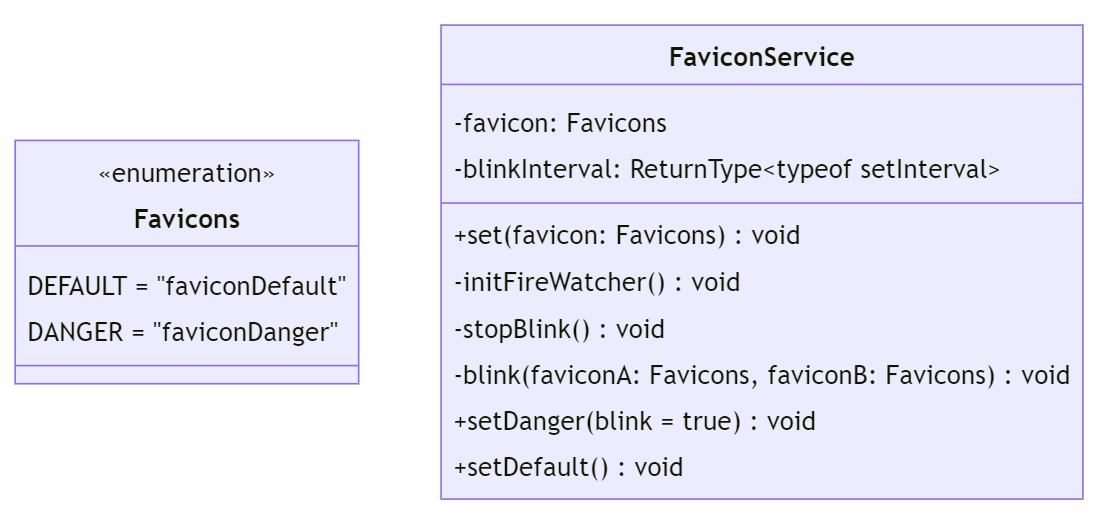
\includegraphics[width=10cm]{class_diagramm_favicon_service}
  \caption{DKlassendiagramm für den Service \lstinline{FaviconService}}
  \label{fig:class_diagramm_favicon_service}
\end{figure}
